\chapter{Week}
The \ac{DPU} integration into the reference designs available for the Mars XU3 and the Mercury+ XU1 continued in this week. For a successful integration the \ac{DPU} user guide was studied and the design adopted to the respective hardware platform. Figure~\ref{fig:dpu_hier} shows an overview over the \ac{DPU} subsystem.
\begin{figure}[!htb]
	\centering
		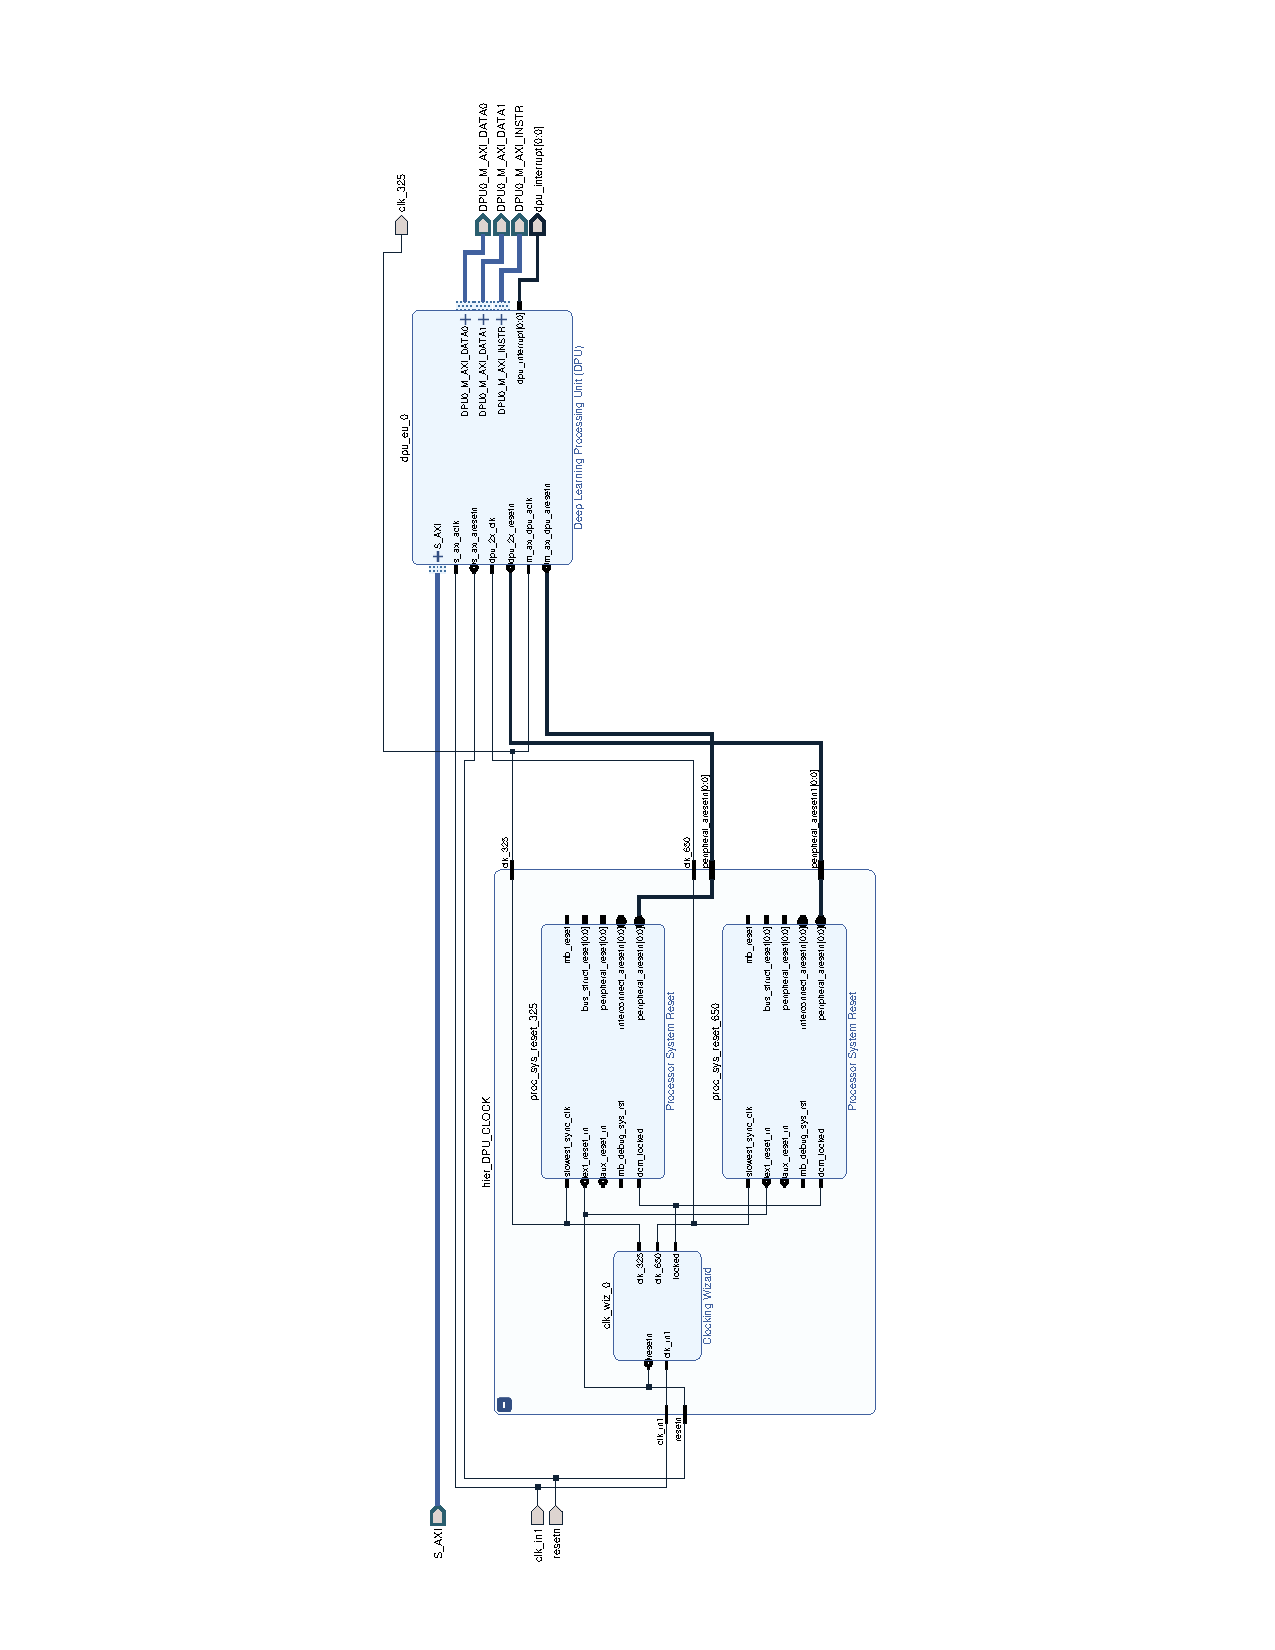
\includegraphics[width=\textwidth]{bilder/dpu_hier.pdf}
		\caption{\acs{DPU} hierarchy system}
		\label{fig:dpu_hier}
\end{figure}
Two main blocks comprise this subsystem: the clock generation and the \ac{DPU} \ac{IP} core itself. For generating the correct clock signals at appropriate frequencies a 'Clocking Wizard' \ac{IP} core is used. This block is configured to take an asynchronous reset and reference clock as input. Internally, a \ac{PLL} is used to generate faster clock frequencies which are needed for the \ac{DPU} \ac{IP} core. As this is a highly optimized hardware block, the frequency can be relatively high compared to the system block. In this design the \ac{DSP} slices are clocked with a frequency of 650 MHz. For each clock signal an asynchronous reset needs to be generated as well. The data exchange of the \ac{DPU} \ac{IP} is handled by \ac{AXI} interfaces.